\documentclass{article}

\usepackage{graphicx}
\usepackage{subfig}
\usepackage{amsmath}
\usepackage{listings}

%\usepackage{amsmath,rotating}

\title{Laminar, Two-dimensional Flow Past Cylinder}

\date{}

\begin{document}

\maketitle

\section{Introduction}
This case provides a description for two-dimensional flow past a cylinder case
with constant properties.

\section{Domain}
The two-dimensional geometry for the midterm assignment is captured in 
Figure~\ref{fig:geom} where a hybrid meshed domain is noted.

The top and bottom surfaces are slip (or zero tangential stress) implemented as a ``symmetry'' boundary 
condition; the left boundary represents an inflow condition specified velocity, $u_x =  U_\infty = 1$. 
The right boundary condition is open, with a specified static pressure. The cylinder wall boundary condition is 
no-slip and specified to be zero. Flow past a rotating cylinder can be modeled by adding a rotational no-slip 
velocity. Properties for density and viscosity are $1.2$ and $0.008$, yielding a Reynolds number of 150 for the unity
sized cylinder diameter.

\begin{figure}[!htbp]
  \centering
  {
   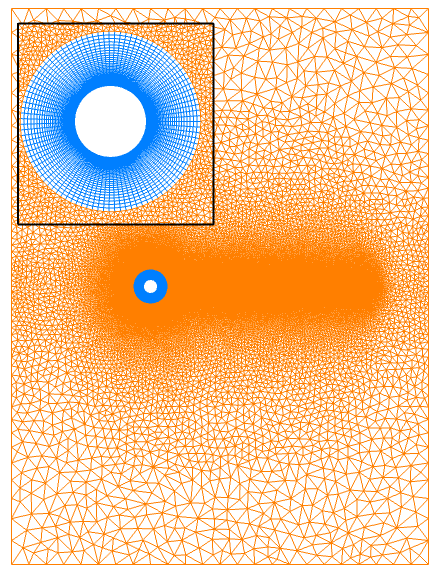
\includegraphics[height=3.0in]{images/street_geom.png}
  }
  \caption{Two-dimensional flow past cylinder hybrid geometry (Quad4 and Tri3) in which the diameter of the cylinder, $D$, is unity.}
  \label{fig:geom}
\end{figure}

\section{Theory}
The variable-density low-Mach equation set is defined by the continuity and momentum equation,

\begin{align}
  \frac {\partial \rho }{\partial t} + \frac{ \partial \rho u_j}{\partial x_j} = 0.
\label{eq:contEq}
\end{align} 

\begin{align}
  \frac {\partial \rho u_i }{\partial t} + \frac{ \partial \rho u_j u_i}{\partial x_j} 
-\frac{\partial \sigma_{ij}}{\partial x_j} = 0.
\label{eq:momEq}
\end{align}
%
In the above equation, $\rho$ is the fluid density and $u_j$ is the fluid velocity. 
The stress tensor is provided by
\begin{align}
\sigma_{ij}  = 2 \mu S^*_{ij} - P \delta_{ij},
\end{align}
%
where the traceless rate-of-strain tensor is defined as
\begin{align}
S^*_{ij}  = S_{ij} - \frac{1}{3} \delta_{ij} S_{kk} \nonumber
		     = S_{ij} - \frac{1}{3} \frac{\partial  u_k }{\partial x_k}\delta_{ij}.
\end{align}
In a low-Mach flow, the above pressure, $P$, is the perturbation about the thermodynamic
pressure, $P^{th}$. The above system can be simplified for a div-free velocity field with constant density.

Although the properties are constant, the baseline case activates a passive scale, $Z$, that is defined as the mixture
fraction. The value of $Z$ varies between zero and unity and can be viewed in an analogous manner as a mass fraction. The transport
of $Z$ is given by,

\begin{align}
  \frac {\partial \rho Z }{\partial t} + \frac{ \partial \rho u_j Z}{\partial x_j} +\frac{\partial q_j}{\partial x_j} = 0,
\label{eq:zEq}
\end{align} 
where $q_j$ is the diffusive flux vector given by $q_j = -\rho D \frac{\partial Z}{\partial x_j}$; $D$ is the diffusivity (units
of $m^2/s)$ whose value is closed by a constant Schmidt number $\rho D = \frac{\mu}{Sc}$. In this particular input file, the
Schmidt number is 0.9, and the value at the cylinder surface is set to unity, while the inflow and open far field entrainment
value is zero. Therefore, the passive scalar $Z$ acts to be transported to highlight the vortical flow exhibited by the 
vortex street. Given that the mixture fraction does not couple to the equations of motion, the boundedness of this variable, i.e.,
the realization of $0.0 \leq Z \leq 1.0$ does not affect the primary flow field. Therefore, modification of this equation's advection
stabilization form (while monitoring the amount of times the variable is clipped),
allows a perspective as to the effectiveness of the stabilization (see the line command $output\_clipping\_diagnostic: yes$).

\section*{Introduction}
The flow of a liquid or gas past a circular cylinder is ubiquitious in
engineering.  Examples include the flow of a river current past a
bridge support column, or wind blowing past a wind turbine tower or
cylindrical water storage tank.  This flow is representative of a
broad class of flows called ``bluff-body'' flows. In a bluff body
flow, the oncoming fluid at first follows the contours of the body,
then at some point separates from the body and creates a wake of
relatively low-momentum fluid behind the body.  This wake is often of
prime importance in engineering of bluff-body systems.  It is
responsible for creation of a large drag force (force opposing the
fluid motion), and can also be responsible for creation of forces on
the body that fluctuate in time (also called unsteady forces).  The
unsteady forces can be oriented both along the wind axis (drag) or
perpendicular to the wind axis (lift).  Unsteady wakes can also be a
source of sound; examples include the wake of aircraft landing gear or
``singing'' power cables in a strong breeze.

The behavior of a bluff-body flow depends on a non-dimensional number
called the Reynolds number.  The Reynolds number is defined as:
\begin{equation}
Re \equiv \frac{\rho~U_\infty~L}{\mu}.
\end{equation}
Here, $\rho$ is the density of the fluid, $U_\infty$ is the oncoming 
fluid velocity relative to the body, or ``free-stream'' velocity, $L$
is a characteristic length scale associated with the size of the body,
and $\mu$ is the fluid viscosity.  For a circular cylinder, $L$ is
usually taken to be the diameter of the cylinder, $D$.  The Reynolds number
can be thought of as the ratio of inertial forces to viscous forces in
a flow.  An example of a low-Reynolds number flow is a marble
dropped in a jar of honey.  An example of a high-Reynolds number flow
is a commercial airliner flying at cruise.  For flows where the
fluid velocity is much smaller than the speed of sound, the Reynolds
number is a similarity parameter; that means any two flows with the
same geometry and same Reynolds number behave exactly the same.

Now, back to the bluff-body wake.  The behavior of this flow can be
dramatically different depending on the Reynolds number.  Take the
circular cylinder.  For very low Reynolds number ($Re < 50$), the flow
is steady; in other words, the fluid velocity at any point in space
near the cylinder does not vary in time.  The wake consists of two
symmetric recirculation regions downstream of the cylinder, as shown
in Figure~\ref{cc_steady}.  As the Reynolds number increases (think of
the fluid speeding up as the cylinder size and fluid properties are
kept the same), the wake behind the cylinder becomes unsteady.
Pockets of swirling fluid, called vortices (plural of vortex), are shed
from the cylinder and are swept downstream.  For $50 < Re < 200$ this
wake remains two-dimensional.  Vortices are shed from either side of
the cylinder in an alternating pattern called a ``vortex street,'' as
shown in Figure~\ref{cc_unsteady}. This shedding phenomenon causes
unsteady lift and drag forces to act on the cylinder at a
characteristic frequency, $f$, called the ``shedding frequency.''  It
is convenient to non-dimensionalize this frequency as follows:
\begin{equation}
  St \equiv \frac{f~D}{U_\infty}
\end{equation}
$St$ is called the Strouhal number, and is a function of the Reynolds
number.
\begin{figure}[h]
\centering
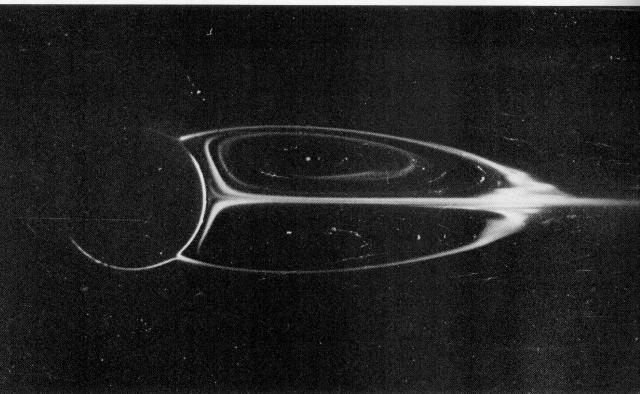
\includegraphics[width=0.575\textwidth]{images/circ_cyl_steady.jpg}
\caption{Flow past a circular cylinder at $Re = 41$, from a flow
  visualization experiment.  The flow is from left to
  right. From Van Dyke, {\em An Album of Fluid Motion}, 1982. \label{cc_steady}}
\end{figure}

\begin{figure}[h!]
\centering
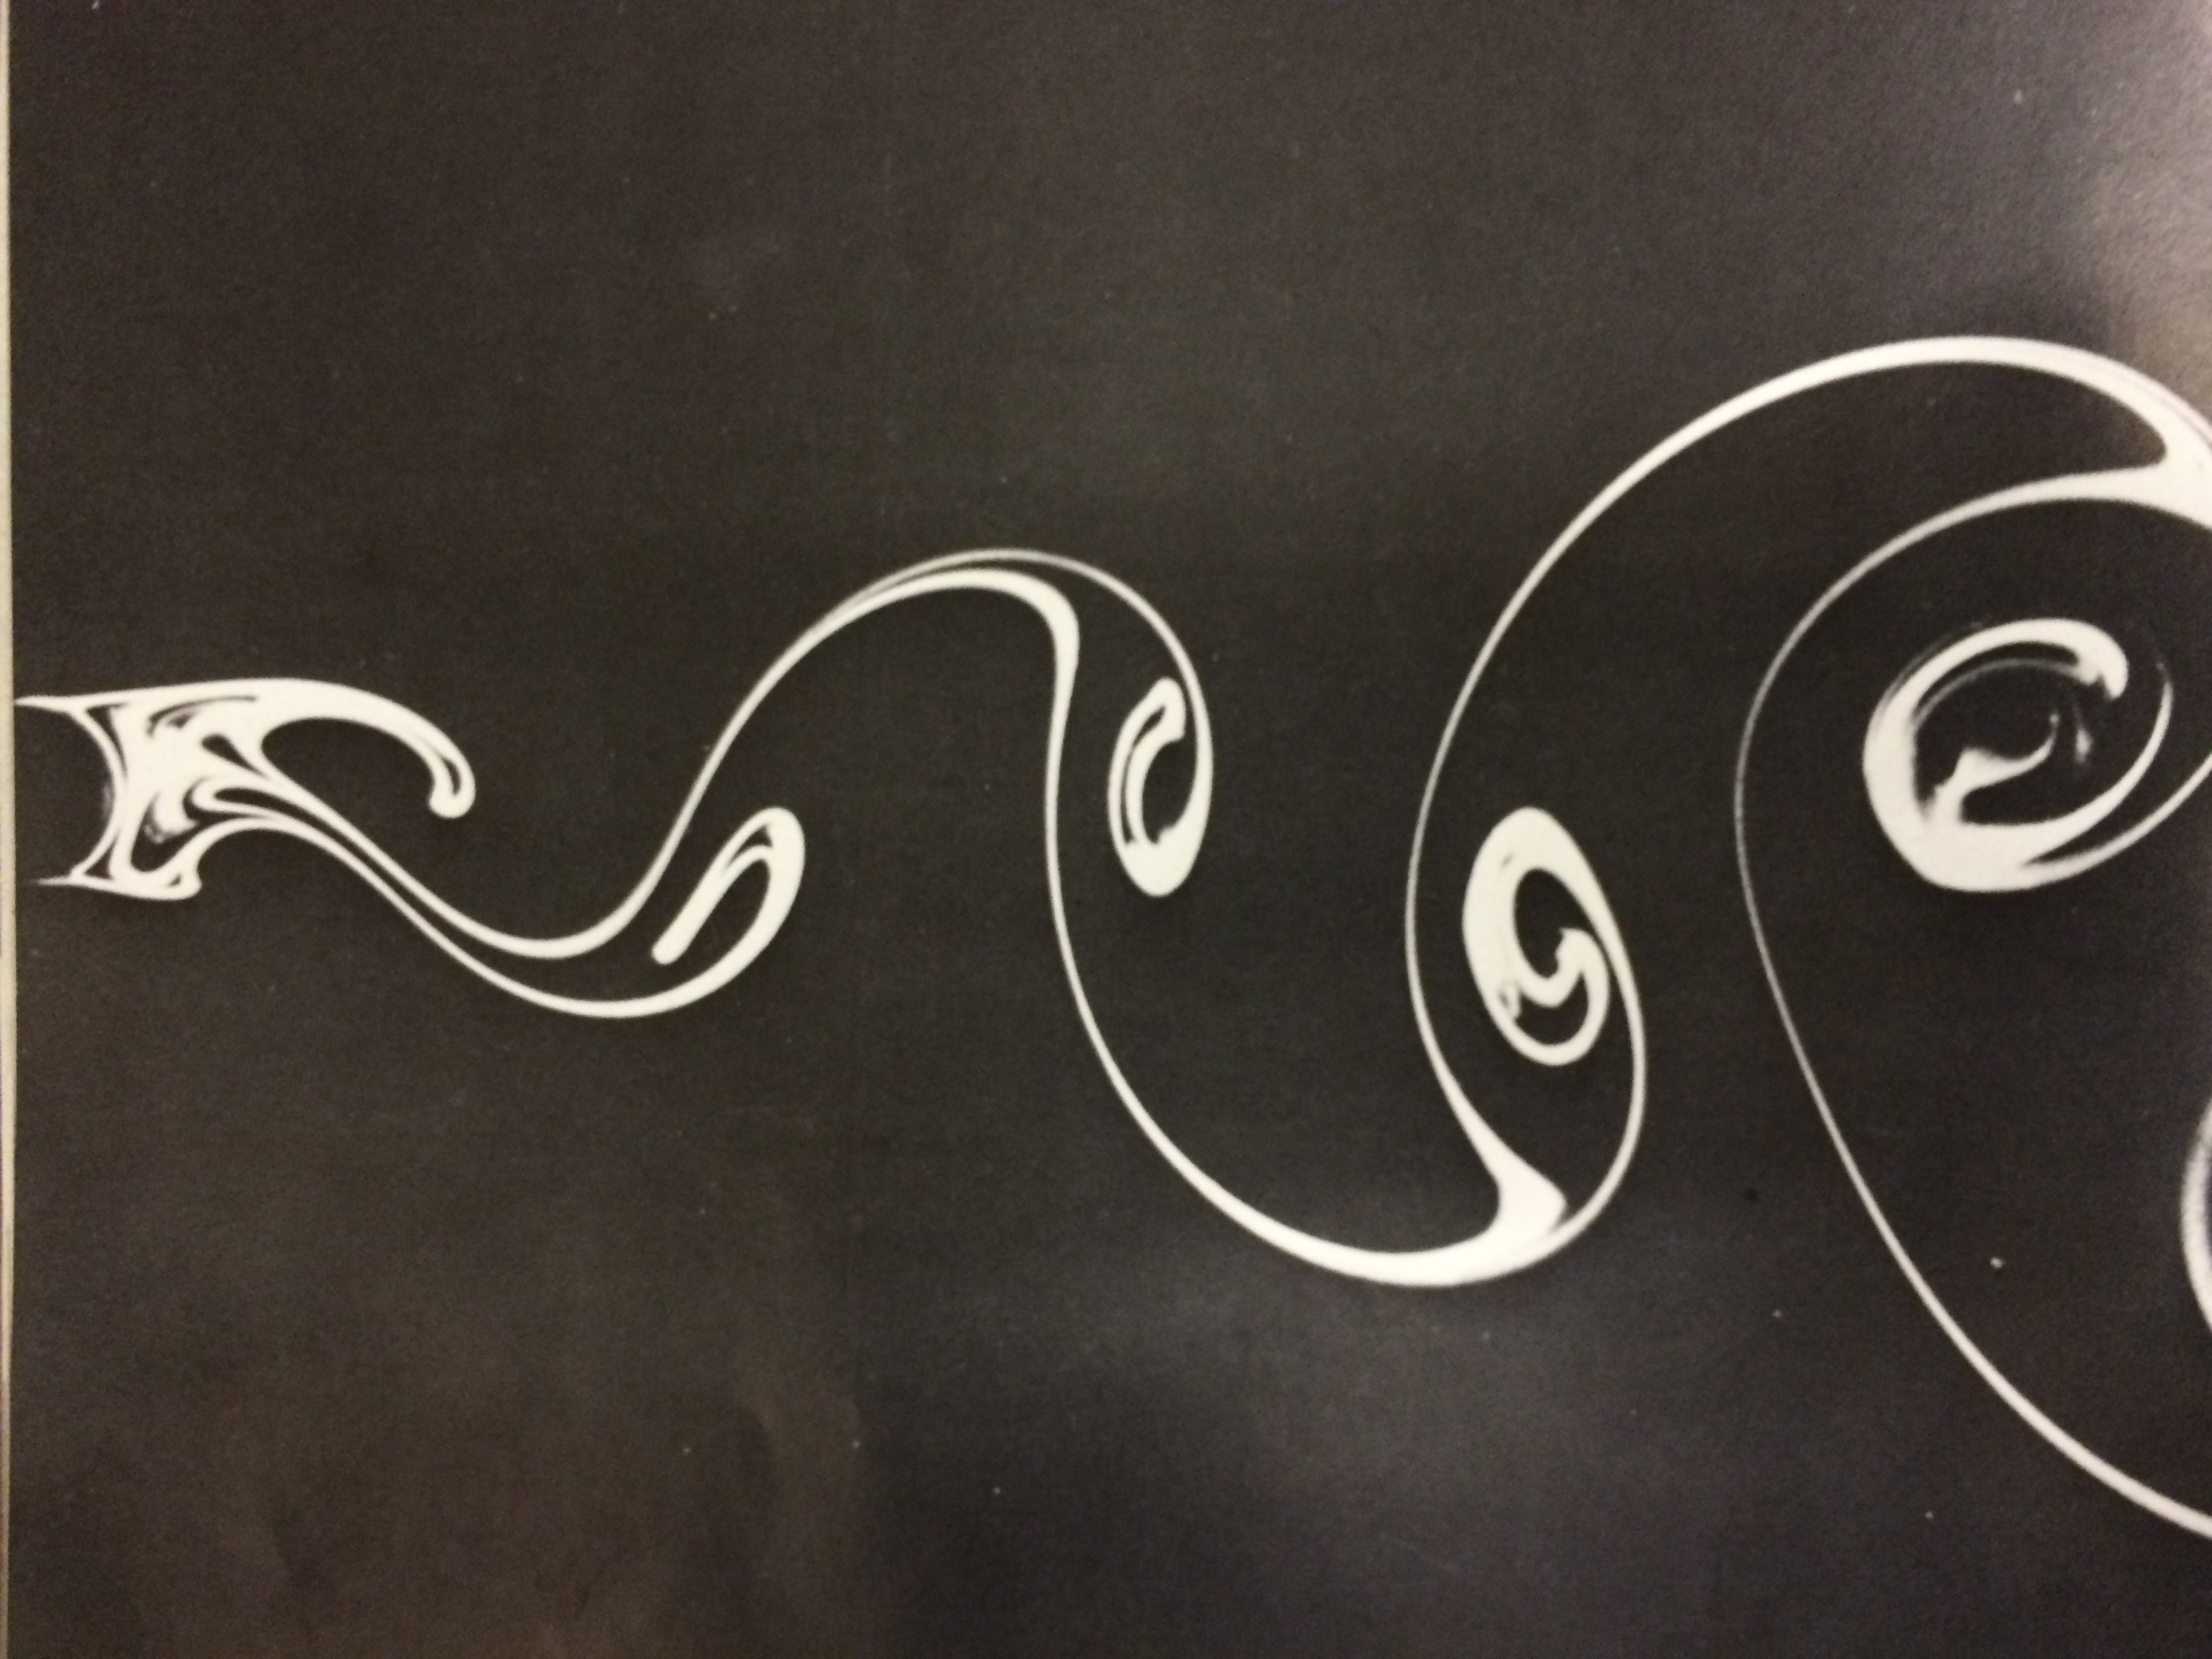
\includegraphics[width=0.575\textwidth]{images/circ_cyl_vandyke.jpg}
\caption{Flow past a circular cylinder at $Re = 140$, from a flow
  visualization experiment.  The flow is from left to
  right. From Van Dyke, {\em An Album of Fluid Motion}, 1982. \label{cc_unsteady}}
\end{figure}


As the Reynolds number continues to increase, more complex flow
behavior is observed.  We will not concern ourselves with the higher
Reynolds number regimes, but the interested reader is encouraged to
investigate this further on their own.

\section*{Quantities of Interest}
In any engineering analysis, we must define the relevant Quantities
of Interest (abbreviated QoI's), which are the analysis outputs that
we are interested in predicting. For the circular cylinder flow, we will
define several:
\begin{itemize}
  \item Time-averaged drag coefficient, $\overline{C_d}$
  \item Strouhal number, $St$
  \item Root-mean-square of the lift coefficient fluctuation,
    $C^\prime_l$
\end{itemize}

We defined the Strouhal number earlier.  The drag coefficient is
defined as:
\begin{equation}
  C_d \equiv \frac{F_d}{1/2 \rho U_\infty^2 D}.
\end{equation}
$F_d$ is the drag force of the fluid acting on the cylinder.  This
force is comprised of two components: the pressure drag, resulting
from the distribution of fluid pressure along the surface of the
cylinder; and the viscous drag, resulting from friction as the fluid
flows past the surface.

Similarly, the lift coefficient is defined as:
\begin{equation}
  C_l \equiv \frac{F_l}{1/2 \rho U_\infty^2 D}.
\end{equation}
$F_l$ is the lift force, or force of the fluid acting in a direction
perpendicular to the oncoming flow.


A sample passive scalar mixture fraction Nalu result for the $Re = 150$ is shown in Figure~\ref{fig:passive_scalar},
while in Figure~\ref{fig:drag_re}, the drag coefficient as a function of Reynolds number, extracted from 
Baracu and Bosneagu (2019), is provided. The coarse mesh for the Nalu simulation is provided for a reference.

\begin{figure}[!htbp]
  \centering
  {
   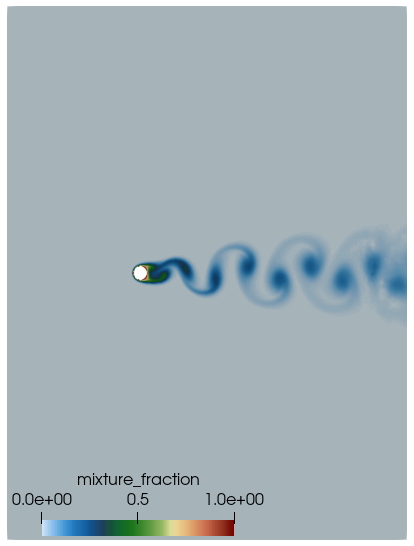
\includegraphics[height=3.0in]{images/vortexStreetR0.png}
  }
  \caption{Two-dimensional passive scalar representation for a $Re = 150$ case in which a Schmidt number of 0.9 is specified to
compute the diffusive flux coefficient.}
  \label{fig:passive_scalar}
\end{figure}

\begin{figure}[!htbp]
  \centering
  {
   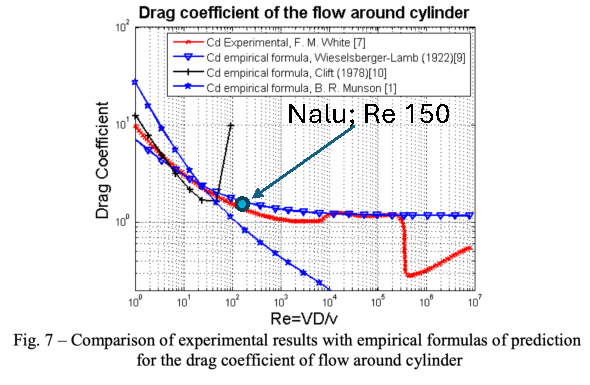
\includegraphics[height=3.0in]{images/cylinder_drag-crop.pdf}
  }
  \caption{Drag coefficient for flow around a cylinder from Baracu and Bosneagu, {\em Scientific Bulletin of Naval Academy, Boll XXII}, 2019.}
  \label{fig:drag_re}
\end{figure}

\section{Discussion Points}

\begin{itemize}
	\item The input file is currently set to terminate only after a small amount of tme steps. While this
              termination may be appropriate for regression testing, for many of the QoIs desired in this
              session, the number of time steps required will be much higher. Please modify accordingly.
	\item Compare timing between EBVC and CVFEM (see command $use\_edges: no$. Comments on speed?
        \item Modify the Reynolds number 10x smaller, 10x larger and report general findings. 
          As you change the Reynolds number, make sure that you adjust the initial time step 
          specification such that the first Courant number reported in the log file is not greater 
          than 2.0.
        \item Explore Peclet blending for both velocity and mixture fraction.
        \item Explore laminar Schmidt number (nominal value of 0.9), 10x smaller; 10x larger.
        \item Monitor the total amount of instances in which the mixture fraction is non-monotonic.
          \subitem The maximum and minimum clipped value can be provided in the MixtureFraction
          equation system via the specification of a deviation from the monotonic range (zero and unity)
          via, $clipping\_delta: 0.0$, where $0.0$ is the current default level. When clipping, how does nonlinear 
          convergence behave?
        \item Explore various quantities of interests (QoIs), including: mean and instant drag 
          coefficient; mean and instant lift coefficient. 
        \subitem Note: $2d\_tri3\_quad4\_street.dat$ 
          that provides forces and moments on the cylinder surface. For QoIs above, at the nominal 
          Reynolds nominal Reynolds number, what is the effect of: a) Mesh refinement; see: 
          $mesh/2d\_tri3\_quad4\_street\_refined.exo$, b) First-order time vs second-order time: 
          $second\_order\_accuracy: yes/no$, c) Changing the number of nonlinear iterations from 2 to 5, 
          and 10: (note the convergence within each step): $max\_iterations: 2, 4, 8$, d) Linear solver 
          tolerance: tolerance: 1e-5, e) Usage of limiters and the effect
        \item (Optional) Compute a FFT for either mixture fraction or velocity at select locations/points in the domain. 
\end{itemize}

\end{document}
